%Version 3.1 December 2024
\documentclass[pdflatex, sn-nature]{sn-jnl}

%%%% Standard Packages
\usepackage{graphicx}%
\usepackage{multirow}%
\usepackage{amsmath,amssymb,amsfonts}%
\usepackage{amsthm}%
\usepackage{mathrsfs}%
\usepackage[title]{appendix}%
\usepackage{xcolor}%
\usepackage{textcomp}%
\usepackage{manyfoot}%
\usepackage{booktabs}%
\usepackage{algorithm}%
\usepackage{algorithmicx}%
\usepackage{algpseudocode}%
\usepackage{listings}%
\usepackage{siunitx}
\usepackage{xr}
\usepackage{cleveref}
%%%%

\crefname{figure}{Supplementary Figure}{Supplementary Figures}
\crefname{table}{Supplementary Table}{Supplementary Tables}
\crefname{section}{Supplementary Note}{Supplementary Notes}

\theoremstyle{thmstyleone}%
\newtheorem{theorem}{Theorem}%
\newtheorem{proposition}[theorem]{Proposition}% 

\theoremstyle{thmstyletwo}%
\newtheorem{example}{Example}%
\newtheorem{remark}{Remark}%

\theoremstyle{thmstylethree}%
\newtheorem{definition}{Definition}%

\graphicspath{{../Image/MS/}}

\externaldocument[supp-]{Supplementary-Information}

\raggedbottom

\begin{document}

\title[]{Spatiotemporal Coherence of Cutaneous Shear Waves, Not Local Extrema, Dictates Mid-Air Tactile Perception}

\author[1]{\fnm{Linhan} \sur{Fan}}\email{linhanfan@seu.edu.cn}

\author[1]{\fnm{Zhutao} \sur{Wang}}\email{xxxx@seu.edu.cn}

\author[1]{\fnm{Hua} \sur{He}}\email{xxxx@seu.edu.cn}

\author*[1]{\fnm{Yafeng} \sur{Niu}}\email{nyf@seu.edu.cn}

\affil*[1]{\orgdiv{School of Mechanical Engineering}, \orgname{Southeast University}, \orgaddress{\city{Nanjing}, \country{China}}}

\abstract{}

\maketitle

\section{Introduction}\label{sec:intro}

Citation Test~\cite{reardonShearShockWaves2023,takahashiTactileStimulationRepetitive2020}

Background of the ultrasound mid-air haptic is presented in \cref{supp-sec:background_umh}.

\section{Results}\label{sec:results}

\begin{figure}
    \centering
    \includegraphics[width=\textwidth]{Figure_Exp.pdf}
    \caption{\textbf{Experimental design and psychophysical evaluation of spatiotemporal modulation patterns.}
        \textbf{a}, Schematic of the experimental setup. Participants were seated with their hand positioned on a hollow foam board over the ultrasound phased array, wearing active noise-canceling headphones playing white noise to eliminate acoustic cues.
        \textbf{b}, Detailed view of the hand-device interface showing the acoustic window and focal alignment.
        \textbf{c}, Illustration of the five modulation patterns ($DLM_2$, $DLM_3$, $ULM_L$, $LM_L$, $LM_C$) and the two-alternative forced choice (2-AFC) protocol. The experiment consisted of two counterbalanced blocks evaluating intensity perception and spatial clarity.
        \textbf{d}, Psychophysical results ($n=26$). Left and Center: Relative preference scores (log-odds) for intensity and spatial clarity derived from a Bayesian mixed-effects Bradley-Terry model. Error bars represent 95\% confidence intervals. Statistical significance is indicated by asterisks (*$P < 0.05$, ***$P < 0.001$; Wald test). Right: Matrix of standardized logarithmic reaction times (Z-Log-RT) for pairwise comparisons, where darker colors indicate longer decision times and higher discrimination difficulty.}
    \label{fig:figure_exp_1}
\end{figure}

\begin{figure}
    \centering
    \includegraphics[width=\textwidth]{Figure_Sim.pdf}
    \caption{\textbf{Elastodynamic simulation of cutaneous shear wave propagation and stress distribution.}
        \textbf{a}, Spatial distributions of peak shear stress in the $xy$-plane for representative modulation patterns ($ULM_L$, $DLM_3$, and $LM_L$), illustrating distinct energy concentration profiles.
        \textbf{b}, Spatiotemporal ($x$-$t$) diagrams of the signed shear stress along the modulation trajectory ($y=0$), visualizing the constructive interference and wave propagation dynamics.
        \textbf{c}, Temporal waveforms of shear stress at the focal center during the steady-state phase (last 15 ms).
        \textbf{d}, Normalized lateral focusing profiles comparing the spatial resolution across all modulation strategies. The full width at half maximum (FWHM) is annotated for each pattern.
        \textbf{e}, Cross-sectional distribution of the root-mean-square (RMS) shear stress along the lateral axis ($y=0$).
        \textbf{f}, Spectral analysis of the induced shear waves (log scale), highlighting the fundamental frequency (200 Hz) and harmonic components generated by different spatiotemporal dynamics.}
    \label{fig:figure_sim_1}
\end{figure}

\begin{figure}
    \centering
    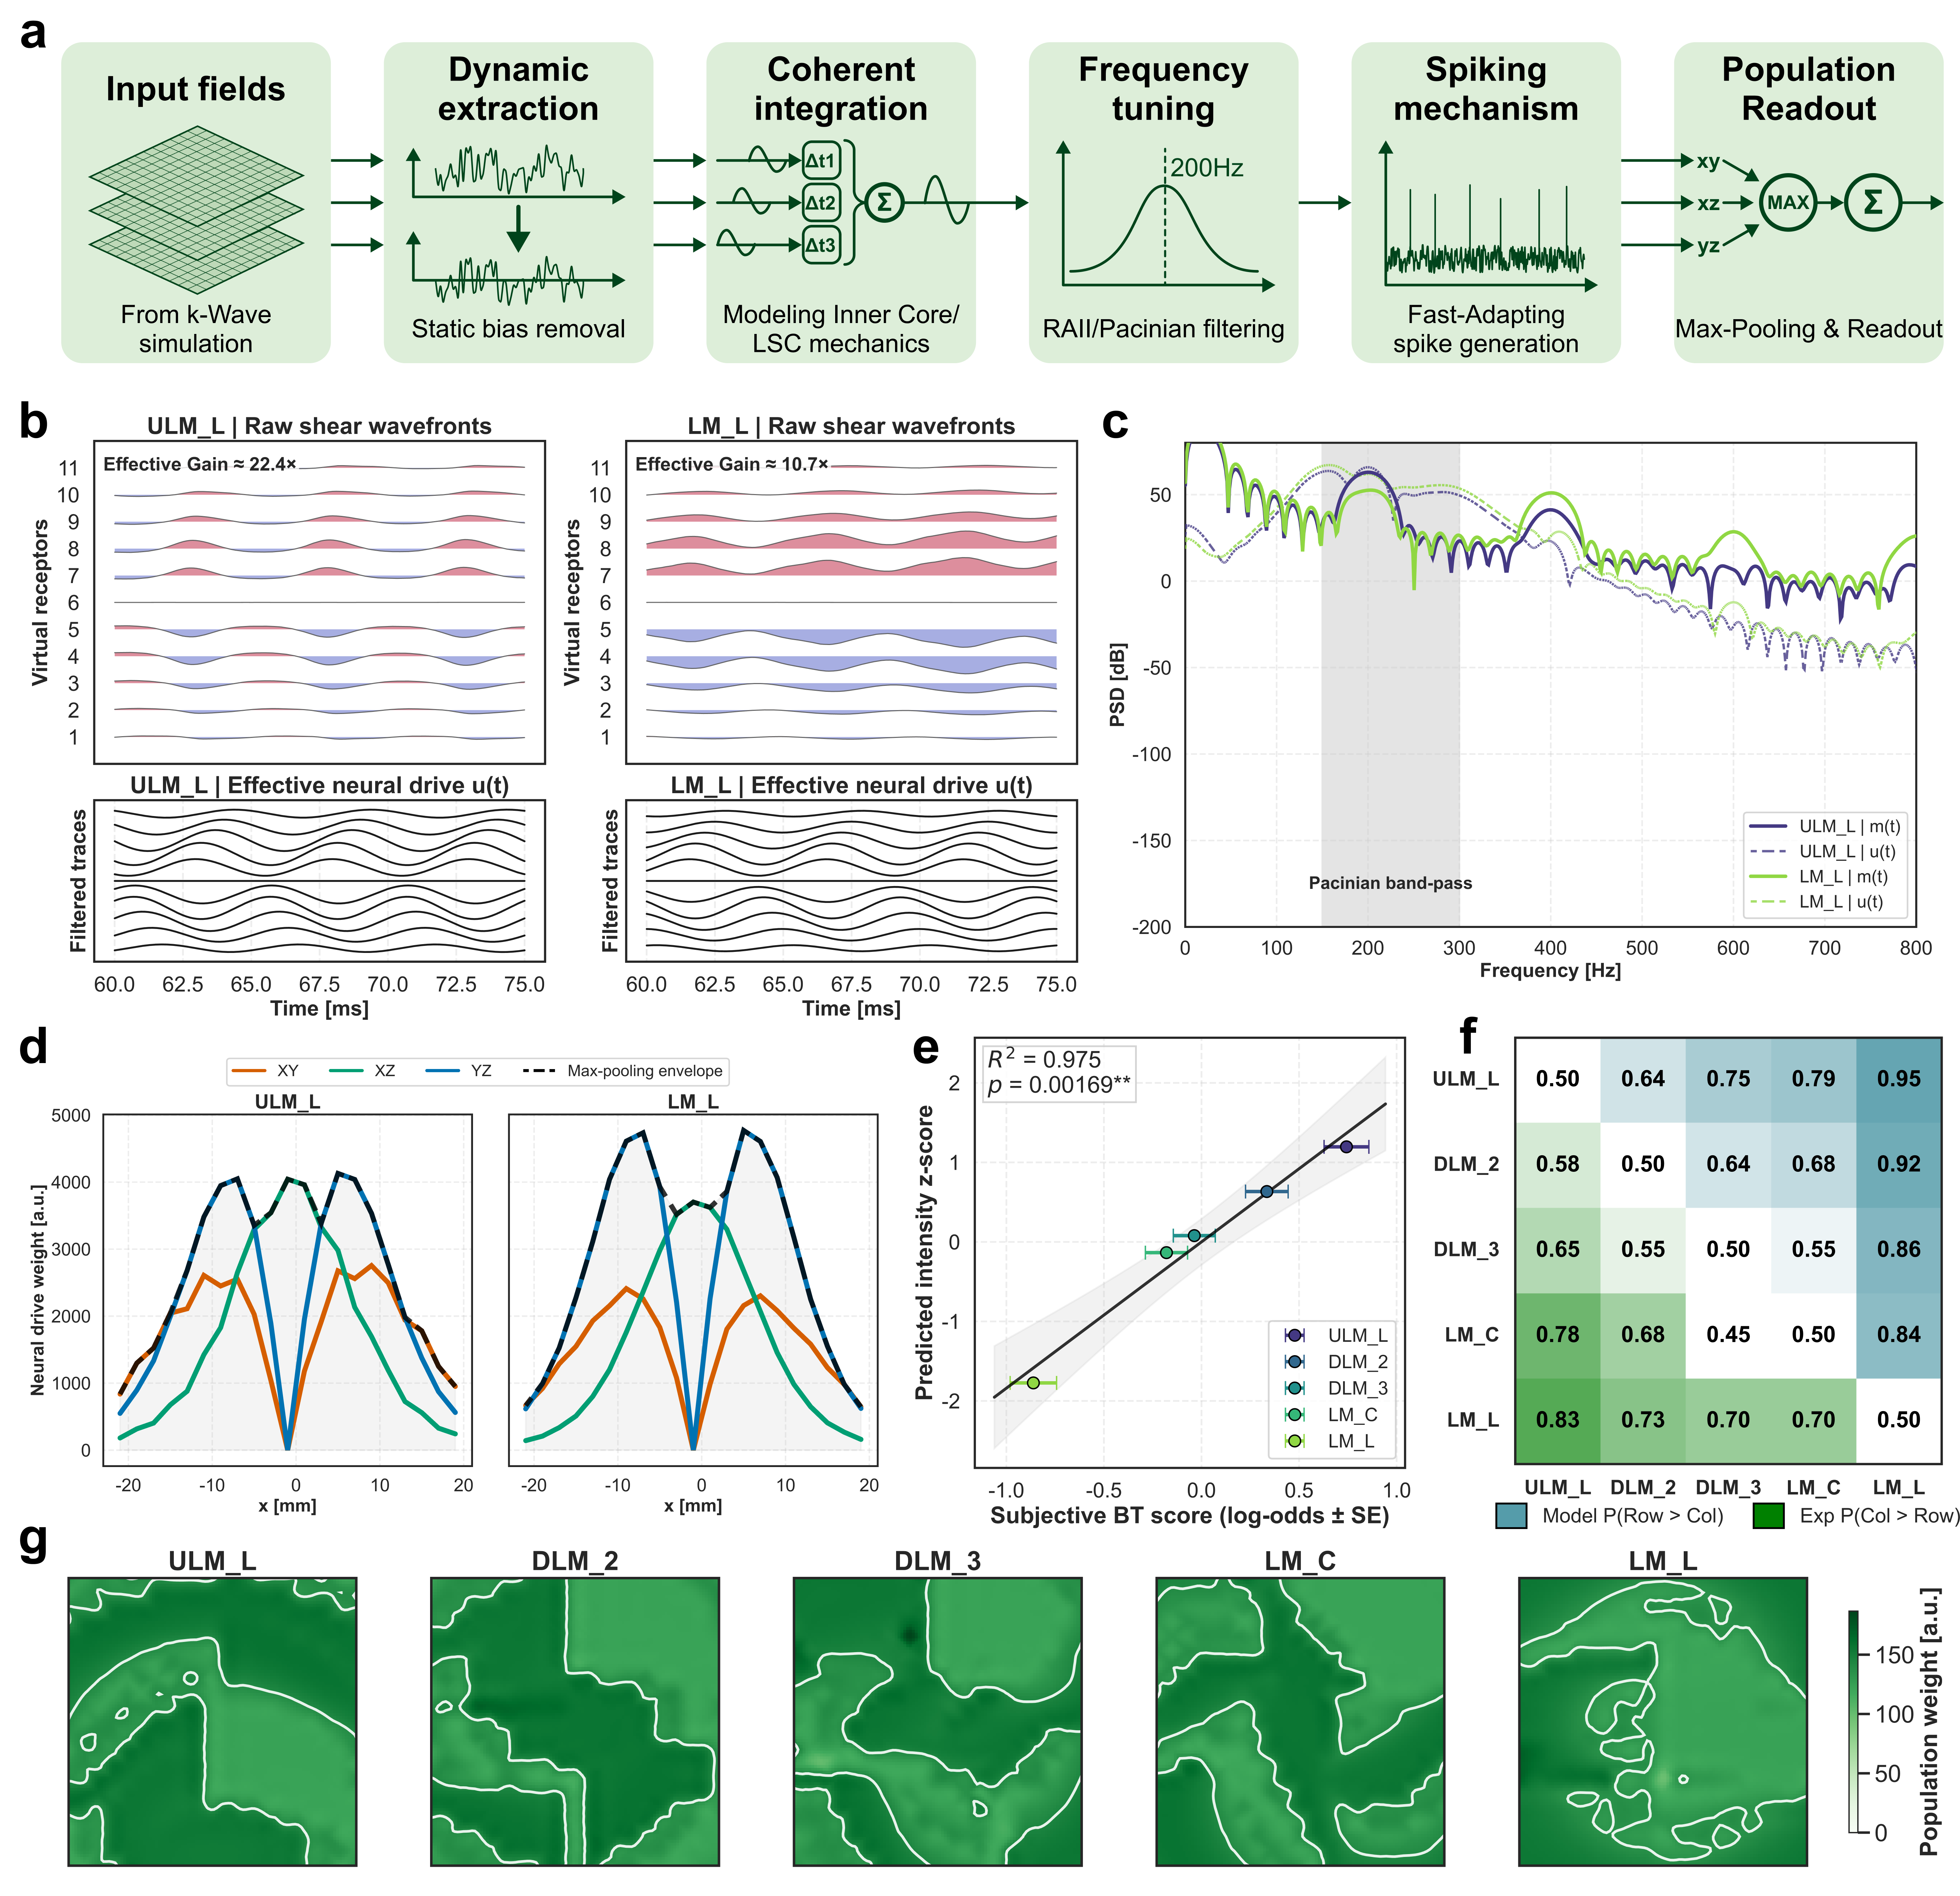
\includegraphics[width=\textwidth]{Figure_Model.pdf}
    \caption{\textbf{.}
        \textbf{a}, .
        \textbf{b}, .
        \textbf{c}, .
        \textbf{d}, .
        \textbf{e}, .
        \textbf{f}, .}
    \label{fig:figure_neural_dynamics_model}
\end{figure}


\section{Discussion}\label{sec:discussion}

\section{Methods}\label{sec:methods}

\backmatter

\section*{Acknowledgments}
This work was supported jointly by National Natural Science Foundation of China (72571059), the SEU Innovation Capability Enhancement Plan for Doctoral Students (CXJH\_SEU 26066).

\bibliography{SWIM}% common bib file

\end{document}
